\documentclass[11pt]{article}
\addtolength{\oddsidemargin}{-1.cm}
\addtolength{\textwidth}{2cm}
\addtolength{\topmargin}{-2cm}
\addtolength{\textheight}{3.5cm}

\usepackage[pdftex]{graphicx}
\usepackage{pdflscape}
\usepackage{hyperref}
\usepackage{float}
\usepackage{cite}
\hypersetup{
	colorlinks=true,
	linkcolor=black,
	filecolor=magenta,
	urlcolor=cyan,
}

% define the title
\author{Team Python}
\title{Architectural Design}

\begin{document}
	\setlength{\parskip}{6pt}
	% generates the coverPage
	\begin{titlepage}
	
	\begin{center}
		% Upper part of the page       
		
\includegraphics[width=0.7\linewidth]{Images/UniLogo.jpg}\\[1cm]    
		\textsc{\LARGE Python Round2}\\[0.3cm]
		
\includegraphics[width=0.5\linewidth]{Images/teamLogo.png}\\[0.5cm]
		% Title
		\rule{\linewidth}{0.5mm} \\[1cm]
		{ \huge \bfseries Architectural Design}\\[0.5cm]
		\rule{\linewidth}{0.5mm} \\[1cm] 			
		
		\begin{minipage}{0.4\textwidth}
			\begin{flushleft} \large
				Dewald {de Jager}
			\end{flushleft}
		\end{minipage}
		\begin{minipage}{0.4\textwidth}
			\begin{flushright} \large
				\emph{} \\
				15188800  
			\end{flushright}
		\end{minipage}
		
		
		\begin{minipage}{0.4\textwidth}
			\begin{flushleft} \large
				\emph{} \\
				Johan {du Plooy}
			\end{flushleft}
		\end{minipage}
		\begin{minipage}{0.4\textwidth}
			\begin{flushright} \large
				\emph{} \\
				12070794
			\end{flushright}
		\end{minipage}
		
		
		\begin{minipage}{0.4\textwidth}
			\begin{flushleft} \large
				\emph{} \\
				Juan {du Preez}
			\end{flushleft}
		\end{minipage}
		\begin{minipage}{0.4\textwidth}
			\begin{flushright} \large
				\emph{} \\
				15189016
			\end{flushright}
		\end{minipage}

		\begin{minipage}{0.4\textwidth}
			\begin{flushleft} \large
				\emph{} \\
				Marthinus {Hermann}
			\end{flushleft}
		\end{minipage}
		\begin{minipage}{0.4\textwidth}
			\begin{flushright} \large
				\emph{} \\
				15081479
			\end{flushright}
		\end{minipage}

		\begin{minipage}{0.4\textwidth}
			\begin{flushleft} \large
				\emph{} \\
				Maria {Qumayo}
			\end{flushleft}
		\end{minipage}
		\begin{minipage}{0.4\textwidth}
			\begin{flushright} \large
				\emph{} \\
				29461775
			\end{flushright}
		\end{minipage}

		\begin{minipage}{0.4\textwidth}
			\begin{flushleft} \large
				\emph{} \\
				Orisha {Orrie}
			\end{flushleft}
		\end{minipage}
		\begin{minipage}{0.4\textwidth}
			\begin{flushright} \large
				\emph{} \\
				13025199 
			\end{flushright}
		\end{minipage}

		\begin{minipage}{0.4\textwidth}
			\begin{flushleft} \large
				\emph{} \\
				Azhar  {Patel}
			\end{flushleft}
		\end{minipage}
		\begin{minipage}{0.4\textwidth}
			\begin{flushright} \large
				\emph{} \\
				15052592 
			\end{flushright}
		\end{minipage}
		
		\textsc{\Large Stakeholders}\\[1cm]	
		
		\begin{minipage}{0.4\textwidth}
			\begin{flushleft} \large
				\emph{} \\
				Computer Science Department of University of Pretoria
			\end{flushleft}
		\end{minipage}
		\begin{minipage}{0.4\textwidth}
			\begin{flushright} \large
				\emph{} \\
				Vreda Pieterse
			\end{flushright}
		\end{minipage}
		
	\end{center}
\end{titlepage}
	\tableofcontents
	\newpage
	
	\section{Introduction}
    \subsection{Purpose}
	\subsection{Scope}
	
	\section{External Interface Requirements}
	\subsection{User Interface}
	\subsection{Hardware Interface}
	\subsection{Software Interface}
	\subsection{Communication}
	
	\section{Performance Requirements}
	\paragraph{The system should be able to run in the following way: }
	\begin{itemize}
	\item The system will be run through campus servers as well as web servers.
	\item The performance of the application will be dependent on the user’s hardware device.
	\item The loading time of each page will be dependent on the strength of the user’s internet connection as well as the number of users currently using campus Wi-Fi.
	\item The time it takes to log in will be dependent on the internet connection.
	\item All new users should be added to the system in less than a second however, it may take the user longer to see this, depending on the internet connection.
	\item Users should be sent notifications as soon as they are available on the system.
	\item Admin should be able to access the GIS module as well as user module with ease in less than a second as these details will be located on campus servers.
	\item Points of interest should appear as soon as a user searches for a location or searches for a specific point of interest however, this will once again be dependent on the internet connection.
	\item Users should be able to search, delete, save as well as modify their route. This should be able to take place quickly. Saving and modifying will be dependent on the user and searching and deleting will be dependent on the internet connection.
	\item Rendering display service will differ from device to device while requesting service relies on the internet connection.
	\item Push services for events should happen as soon as the event has been added to the application
	\item Fitness service and heat maps should be updated in real time.
	\end{itemize}
	
	\section{Design Constraints}
	
	\section{Software System Attributes}
	\subsection{Reliability}
	When transferring data from point A to point B, it is crucial that the integrity of every piece of information be maintained and accounted for.  One piece of misinformation could very well mean the difference between the locations of two different class rooms or even completely different buildings.  One of the applications features is to ensure the fastest route, which relies heavily on making the right decisions based on the data it receives, therefore if the information is not accurate or even correct, the user could end up late to their desired destination.
	\subsection{Robustness}
	All functionality of NavUP must work correctly even under exceptional conditions; The most important being correctness when there is no Wi-Fi connection, extremely slow Internet connectivity or low availability of resources on either the host system for each access channel or the server.
	
	The data module should provide means of communication even when the server is under strain in order to be robust. This may be done in terms of a pipeline system where messages are queued and receipt of them are acknowledged, along with the error detection and correction discussed under Reliability.
	\subsection{Efficiency}
	Sending data between remote locations relies heavily on the network traffic and its capabilities/limitations.  Thus the idea would be to put the least amount of stress and congestion on that network and only make strategic requests from client to server.  The idea would be to make relatively frequent requests to small yet crucial information, and much less frequent requests to information that is less likely to change within a small period of time.
	\subsection{Interoperability}
	\subsection{Maintainability}
	\subsection{Testability}
	\subsection{Portability}
	\subsubsection{Hardware Independence}
	Seeing as how the system will be deployed with a web base as a back-end API, the hardware choices are not limited to a specific set of components, so long as they meet the minimum or preferably recommended requirements to be able to handle the estimated network traffic to keep the system performing at optimal levels.
	\subsubsection{Software Dependence}
	The software on the other hand will be limited to being web specific, i.e. being able to use or integrate with applications like AJAX, Node etc.
	\subsection{Reusability}
	\subsection{Modularity}
	\subsection{Cohesion}
	The NavUP system can be designed with the high cohesion principle in mind.  The system as a whole should be formulated in to a hierarchical tree-structure, comprising of subsystems, or modules.  The modules should be able to either function independently, or be able to call on one or more modules in the hierarchy to perform a given task.  Thus adding or removing modules should not break the system so much as increase or reduce  its functionality as a whole.
	
	The Data module comprises mainly out of a client and a server subsystem.  The server for example would be able to make use of a Database Management System, for handling records relevant to the NavUP system, such as location information, events etc.  Furthermore, both the Client and Server would need to have some form of communication method, which could also be in the form of a subsystem or module.
	\subsection{Coupling}
	The subsystems should have minimal impact on and dependency on the other subsystems of the system. The system as a whole applies the low coupling principle. Subsystems should be abstracted and implementation changes should only affect the subsystem that was modified. This abstraction layer will provide an interface between all the subsystems that prevents interference and augments communication between them.
	
	The data module will be represented as a module with requests and responses that are used both by access channels and the server. This allows for other subsystems to easily use it without having to worry about implementation specific details and the implementation can be changed to use a different technology or update the application programming interface (API).
	
	\section{Technologies}
	\subsection{Data}
	Message passing is done in a transactional manner in this subsystem. The access channels, or clients, need a way to send requests to the server and receive responses. Likewise, the server needs a way to service requests and issue responses. The University of Pretoria Wi-Fi infrastructure can be advantageous in this scenario as we can assume the user is likely connected to the Wi-Fi and fall back on cellular data otherwise. This is done by having the server accessible both locally and publicly via the Internet. If a connection cannot be established to the local server a connection via cellular data or a different Wi-Fi connection is made to the server.
	
	The connection is established via either the HyperText Transfer Protocol (HTTP), or it's secured counterpart HTTPS that makes use of the Secure Socket Layer (SSL) depending on the nature of the message contents, and is maintained only for the duration of the message send and receive process. The requests will, more specifically, be made using Asynchronous JSON and XML (AJAX) and will always be paired with a response. The protocol that HTTP is built on, the Transmission Control Protocol (TCP), ensures the delivery of messages in the correct order and that the messages remain intact.
	\subsection{Users}
	\subsection{Events}
	\subsection{Points of Interest}
	
	\section{UML Diagrams}
	\subsection{Data}
	\begin{figure}[!h]
        \centering
        \includegraphics[width=\textwidth]{Diagrams/Data/data_use_case_diagram}
        \caption{Data Use Case Diagram}
        \label{fig:data_use_case}
    \end{figure}
    \begin{figure}[!h]
        \centering
        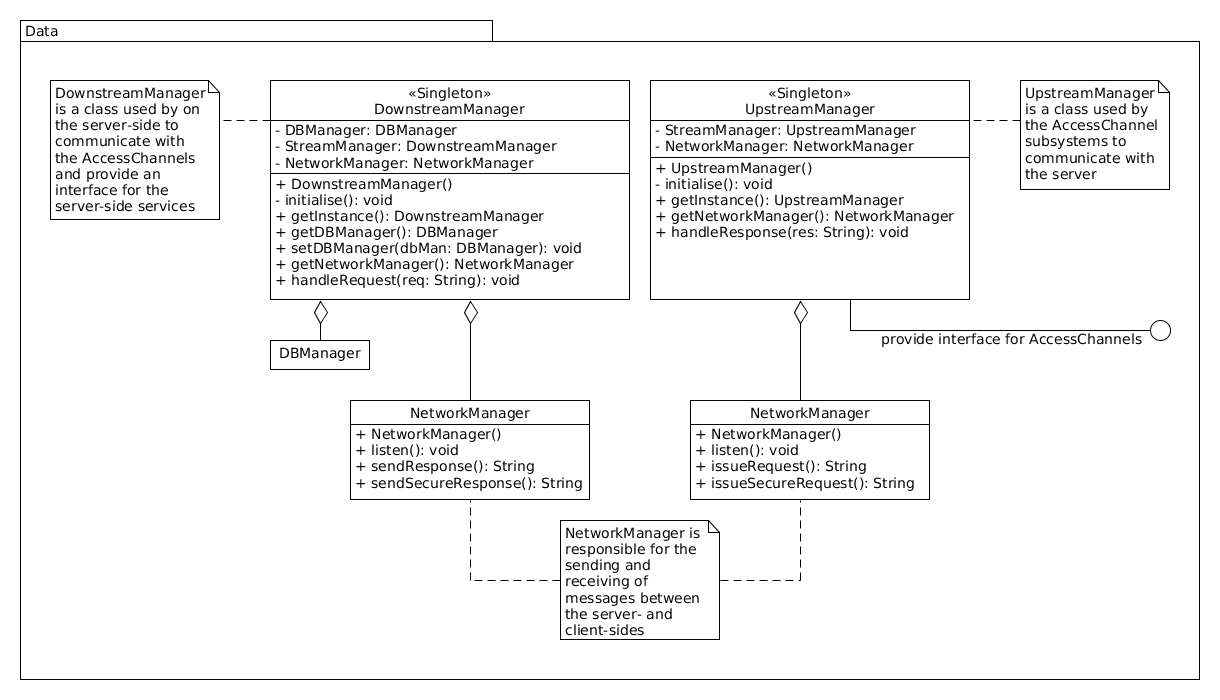
\includegraphics[width=\textwidth]{Diagrams/Data/data_class_diagram}
        \caption{Data Class Diagram}
        \label{fig:data_class}
    \end{figure}

	\subsection{Users}
	\begin{figure}[!h]
        \centering
        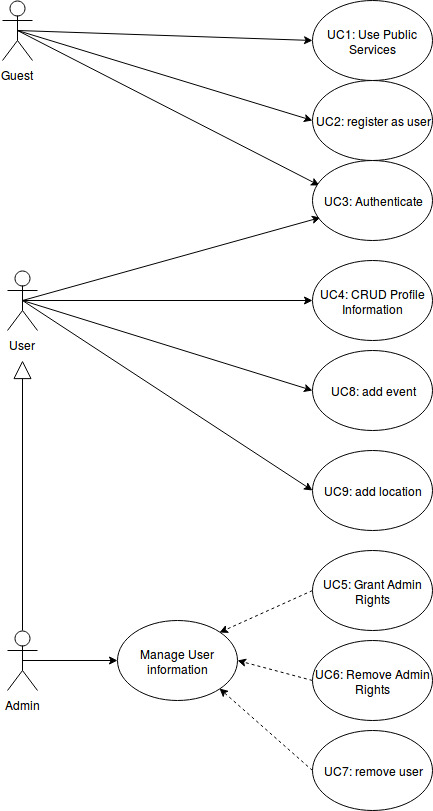
\includegraphics[width=\textwidth]{Diagrams/UserManagement/UserUseCaseDiagram}
        \caption{User Management Use Case Diagram}
        \label{fig:user_use_case}
    \end{figure}
    \begin{figure}[!h]
        \centering
        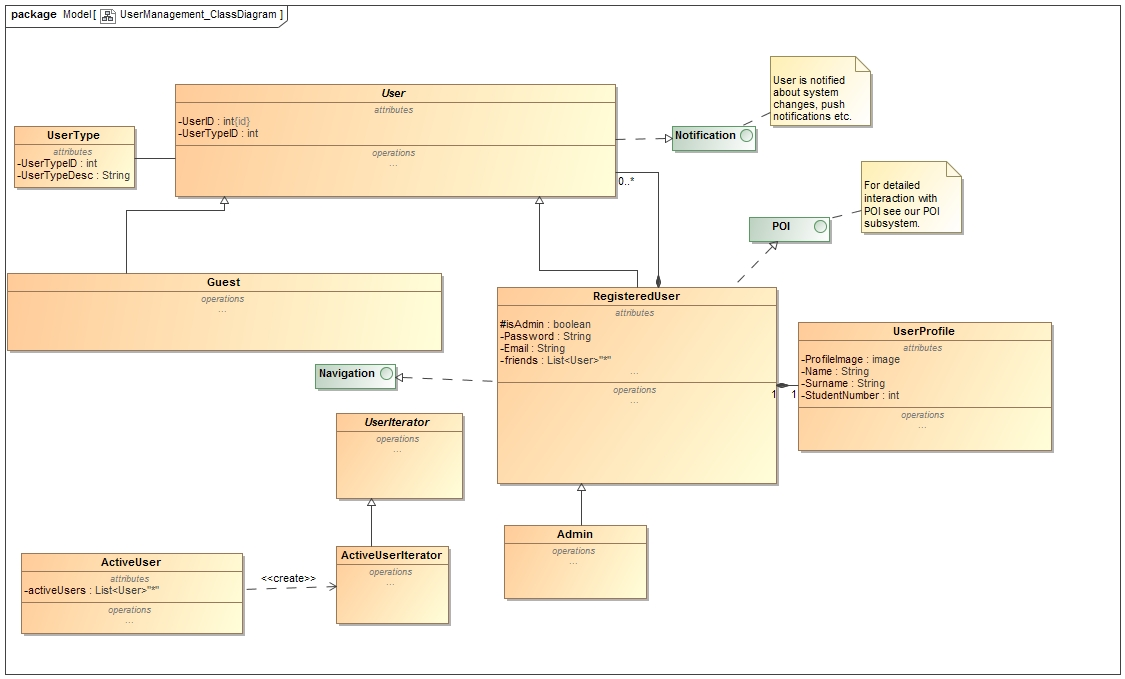
\includegraphics[width=\textwidth]{Diagrams/UserManagement/UserManagement_ClassDiagram}
        \caption{User Management Class Diagram}
        \label{fig:user_class}
    \end{figure}
    \begin{figure}[!h]
        \centering
        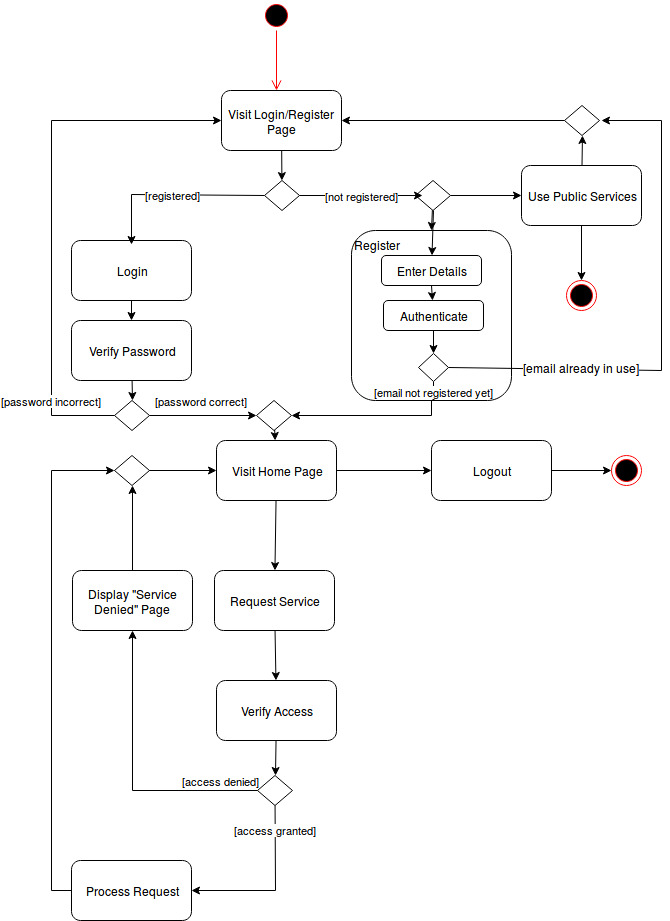
\includegraphics[width=\textwidth]{Diagrams/UserManagement/UseActivityDiagram}
        \caption{User Management Activity Diagram}
        \label{fig:user_activity}
    \end{figure}
	\subsection{Events}
	\begin{figure}[!h]
        \centering
        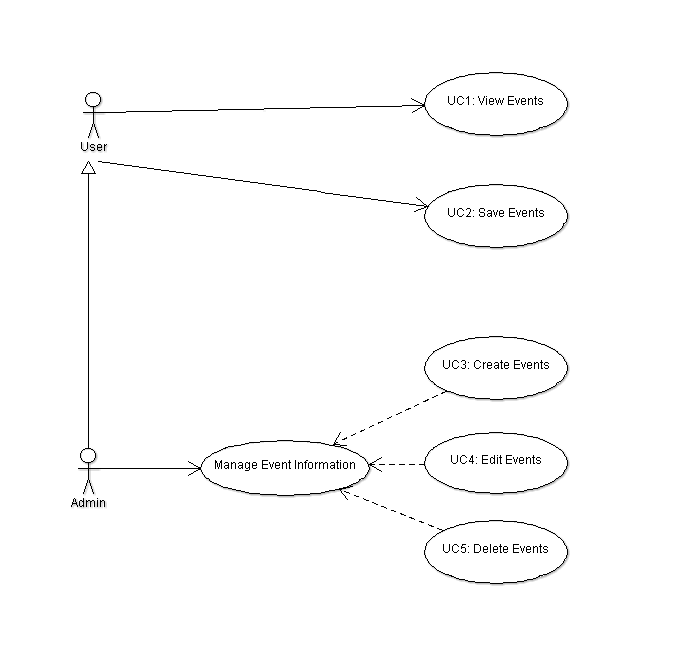
\includegraphics[width=\textwidth]{Diagrams/Events/AzharEventsUseCaseDiagram}
        \caption{Events Use Case Diagram}
        \label{fig:events_use_case}
    \end{figure}
    \begin{figure}[!h]
        \centering
        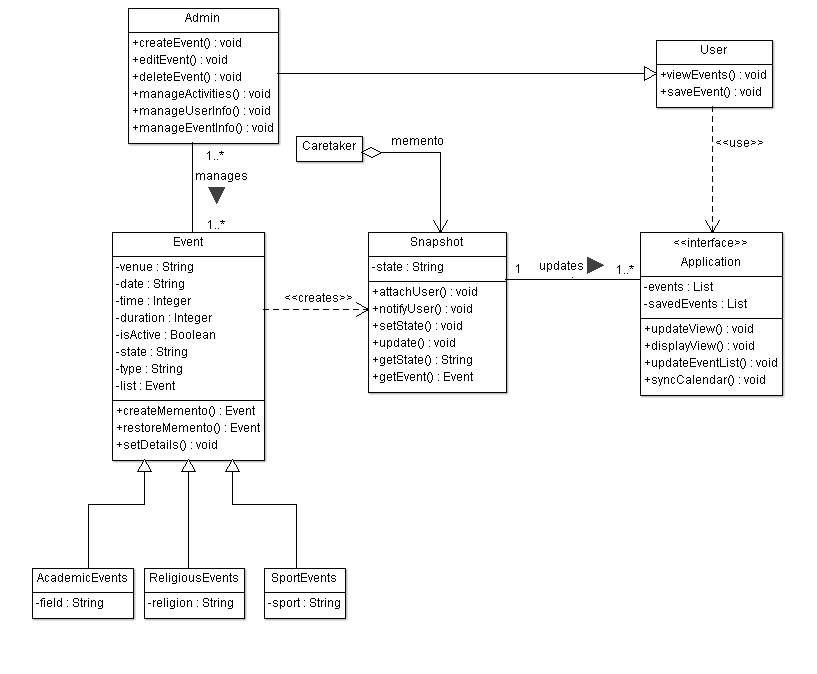
\includegraphics[width=\textwidth]{Diagrams/Events/AzharEventsClassDiagram}
        \caption{Events Class Diagram}
        \label{fig:events_class}
    \end{figure}
	\subsection{Points of Interest}
	\begin{figure}[!h]
        \centering
        \includegraphics[width=\textwidth]{Diagrams/PointsOfInterest/"Placesofinterest (1)"}
        \caption{Points of Interest Use Case Diagram}
        \label{fig:poi_use_case}
    \end{figure}
    \begin{figure}[!h]
        \centering
        \includegraphics[width=\textwidth]{Diagrams/PointsOfInterest/"POIClass (6)"}
        \caption{Points of Interest Class Diagram}
        \label{fig:poi_class}
    \end{figure}
\end{document}
